\documentclass[lettersize,journal]{IEEEtran}
\usepackage{amsmath,amsfonts}
\usepackage{algorithm}
\usepackage{algpseudocode}
\usepackage{array}
\usepackage[caption=false,font=normalsize,labelfont=sf,textfont=sf]{subfig}
\usepackage{textcomp}
\usepackage{stfloats}
\usepackage{url}
\usepackage{verbatim}
\usepackage{graphicx}
\usepackage{cite}
\hyphenation{op-tical net-works semi-conduc-tor IEEE-Xplore}
% updated with editorial comments 8/9/2021

% 自定义命令
\newcommand{\ie}{\textit{i.e.}}
\newcommand{\etc}{\textit{etc.}}
\newcommand{\etal}{\textit{et~al.~}}
\newcommand{\eg}{\textit{e.g.}}
\newcommand{\cf}{\textit{c.f.}}
\algrenewcommand\alglinenumber[1]{\scriptsize #1}
\newcommand{\algstep}[2]{\State \makebox[1.8em][r]{\scriptsize #1}\quad #2}


\begin{document}

    \title{Remote Sensing Changing Detection with\\ Fake Changing Suppressing}
    
    \author{
        Guixin Lv,$^{1,2}$,
        Ziyou Guo$^{1,2}$,
        Ruyue Feng$^{2}$,
        Tieru Wu$^{2,*}$,
        Xiao Du$^{3,*}$    
        \thanks{$^{1}$These authors contribute to this paper equally.}
        \thanks{$^{2}$These authors are with the School of Artificial Intelligence, Jilin University, Changchun City, Jilin Province, China. Email: lvgx24@mails.jlu.edu.cn, guozy22@mails.jlu.edu.cn, fengry21@mails.jlu.edu.cn, wutr@mail.jlu.edu.cn}
        \thanks{$^{3}$These authors are with the School of Mathematics, Jilin University, Changchun City, Jilin Province, China. Email: duxiao18@mails.jlu.edu.cn}
        \thanks{$^{*}$Corresponding authors.}
    }    
    
    % The paper headers
    \markboth{Journal of IEEE Transactions on Geoscience and Remote Sensing ~Vol.~XX, No.~X, August~202X}%
    {Shell \MakeLowercase{\textit{et al.}}: Remote Sensing Changing Detection with Fake Changing Suppressing}
    
    \IEEEpubid{0000--0000/00\$00.00~\copyright~2021 IEEE}
    % Remember, if you use this you must call \IEEEpubidadjcol in the second
    % column for its text to clear the IEEEpubid mark.
    
    \maketitle    
    
    % 摘要和关键词
    \input{Sections/0-Abstract}
    
    % 引言
    \section{Introduction}\label{sec:Introduction}
    \IEEEPARstart{T}{his} is the introduction.
    
    % 相关工作
    \section{Related Work}\label{sec:RelatedWork}
    Remote sensing change detection is closely related to visual representation learning, bi-temporal feature comparison, pseudo-change suppression, and dense prediction. This section reviews representative studies from these four aspects.

    \subsection{Visual Representation Learning for Remote Sensing}\label{sec:RelatedWork:Vision}
        Remote sensing imagery contains complex spatial structures, spectral responses, and scale variations, which makes robust visual representation learning essential for downstream interpretation. Ji \etal proposed PASSNet\cite{passnet} with a patch attention module for hyperspectral image classification. Han \etal studied optical remote sensing object detection using weakly supervised learning and high-level feature learning\cite{weakly-supervised}. Wang \etal designed FSoD-Net\cite{Full-scale} for full-scale detection in optical remote sensing imagery. Liu \etal investigated unsupervised contextual anomaly detection for remotely sensed data\cite{unsupervised}. Xiao \etal introduced a diffusion-based super-resolution model for remote sensing images\cite{diffusion}. These studies improve remote sensing representation from classification, detection, anomaly modeling, and restoration perspectives, but they mainly operate on single images. In contrast, change detection requires discriminative representation as well as explicit comparison between two temporal observations.

    \subsection{Bi-Temporal Remote Sensing Change Detection}\label{sec:RelatedWork:ChangeDetection}
        Deep change detection methods usually learn bi-temporal representations with siamese or dual-stream architectures. Daudt \etal introduced fully convolutional siamese networks as an early deep comparison framework\cite{fully-rs}. Fang \etal further improved siamese modeling through dense connections in SNUNet-CD\cite{Siamese-network}. Long \etal proposed SASiamNet\cite{Self-adaptive-Siamese-network} with self-adaptive feature interaction in a siamese framework. Peng \etal combined attention mechanisms with image differencing for change detection\cite{attention-sample}. Wang \etal introduced attention-based deep supervision in ADS-Net\cite{deeply-supervised-network}. Gu \etal focused on full-scale difference feature fusion in FDFF-Net\cite{full-scale-difference-feature-fusion-network}. Wang \etal proposed a high-resolution feature difference attention network for building change detection\cite{feature-difference-attention-network}. Chen \etal introduced transformer-based modeling for remote sensing change detection\cite{transformers-rs}. Ma \etal presented EATDer\cite{ma2023eatder} with edge-assisted adaptive transformer detection. Li \etal further combined semantic flow and edge-aware refinement in SFEARNet\cite{sfearnet} to improve efficient change reasoning. Although these methods have advanced bi-temporal fusion and boundary localization, many of them still treat visual discrepancy as the main evidence of change, which may lead to false responses in pseudo-change regions.
        
    \IEEEpubidadjcol
    
    \subsection{Pseudo-Change Suppression in Change Detection}\label{sec:RelatedWork:PseudoChange}
        Pseudo-change refers to visually apparent differences that are not annotated as semantic changes. It is commonly caused by illumination variation, seasonal transition, sensor inconsistency, atmospheric interference, or local imaging conditions. Zhang and Xue proposed SIAM-CDNET\cite{optimized-edge-detection} to optimize edge detection and mitigate pseudo changes. Cheng \etal introduced a content-cleansing framework to remove unreliable cues before change inference\cite{harmony}. Chen \etal formulated building change detection as an XOR-style binary relation problem\cite{buildings}. Wang \etal proposed FIBTNet\cite{Feature-Interactive} to enhance feature interaction between bi-temporal observations. These methods share the view that pseudo-change cannot be fully handled by simple appearance differencing and requires stronger semantic or structural constraints.

        Semi-supervised and contrastive learning methods also provide useful insights for pseudo-change suppression. Sun \etal explored semi-supervised change detection with siamese networks and graph attention\cite{semisanet}. Kondmann \etal proposed SemiSiROC\cite{SemiSiROC} with an unsupervised teacher model. Wang \etal proposed reliable contrastive learning to separate changed and unchanged representations\cite{contrastive-learning}. Wang \etal introduced STCRNet\cite{self-training} with self-training and consistency regularization. These methods improve robustness by exploiting unlabeled data, consistency constraints, or representation separation. However, the core challenge of pseudo-change remains the inconsistency between visual difference and annotation semantics. Therefore, an annotation-consistent supervision strategy is still needed to guide the model toward benchmark-defined changes rather than all observable differences.

    \subsection{Dense Prediction and Semantic Segmentation in Remote Sensing}\label{sec:RelatedWork:DensePrediction}
        Dense prediction methods provide important design references for pixel-wise change detection, especially in foreground modeling and boundary delineation. As a semantic-segmentation reference, Xu \etal proposed RSSFormer\cite{rssformer} to enhance foreground saliency for remote sensing land-cover segmentation. Tang \etal developed WNet\cite{wnet} with a hierarchical W-shaped structure for remote-sensing image change detection. Yuan \etal improved multi-scale feature modeling through the global filter in the frequency domain\cite{multi-scale}. Lu \etal proposed a multi-scale feature progressive fusion network for change detection\cite{multi}. Ma \etal introduced edge-assisted adaptive transformer detection\cite{ma2023eatder}. These methods show that accurate dense prediction benefits from foreground saliency, multi-scale context, and boundary-aware refinement. Nevertheless, semantic segmentation is usually single-temporal, whereas change detection must compare two temporal observations and distinguish semantic change from pseudo-change. Thus, segmentation-related techniques are useful components, but they do not by themselves solve annotation-consistent bi-temporal change detection.

    
    % 预备知识
    \section{Preliminary}\label{sec:Preliminary}
    % 写预备知识，主要是别人的论文里面的已经提出的方法、技术、或者损失，在本文中要用到。但是明确不是自己提出的。
    % 写一段简短的开场白。注意，这里开始，给每个东西所使用的名字、数学符号，就得定好，后续方法章节也得统一符号明明。最好给出一个表格，实时记录每个变量的含义。
    \subsection{Notations}\label{sec:Preliminary:Notations}
        To avoid ambiguity, the main symbols used in this paper are summarized in Table~\ref{tab:notations}. Their definitions are fixed throughout the remainder of the manuscript.

        \begin{table}[t]
            \centering
            \caption{Summary of the main symbols used in this paper.}
            \label{tab:notations}
            \footnotesize
            \setlength{\tabcolsep}{4pt}
            \renewcommand{\arraystretch}{1.15}
            \begin{tabular}{>{\raggedright\arraybackslash}p{0.28\columnwidth}>{\raggedright\arraybackslash}p{0.62\columnwidth}}
                \hline
                Symbol & Meaning \\
                \hline
                $\mathbf{I}^{t_1}, \mathbf{I}^{t_2}$ & Bi-temporal input images captured at times $t_1$ and $t_2$. \\
                $\hat{\mathbf{Y}}$ & Predicted binary change map. \\
                $\mathbf{Y}$ & Ground-truth binary change map. \\
                $\mathbf{Y}^{e}$ & Ground-truth edge supervision map. \\
                $\mathbf{P}\in\mathbb{R}^{2\times H\times W}$ & Change prediction logits. \\
                $\mathbf{P}^{e}\in\mathbb{R}^{2\times H\times W}$ & Edge prediction logits. \\
                $\mathbf{F}^{t_1}, \mathbf{F}^{t_2}\in\mathbb{R}^{C\times H\times W}$ & Deep feature maps extracted from the two temporal observations. \\
                $\mathcal{N}_{\theta}$ & Change detection network parameterized by $\theta$. \\
                $\Omega=\{1,\ldots,H\}\times\{1,\ldots,W\}$ & Spatial domain of an image. \\
                $(i,j)\in\Omega$ & Pixel location at row $i$ and column $j$. \\
                $p^{1}_{b,ij}, q^{1}_{b,ij}$ & Foreground probabilities of the change and edge branches after softmax. \\
                $B$ & Batch size. \\
                $\alpha$ & Balance factor between CE loss and IoU loss within the segmentation branch. \\
                $\beta$ & Weight of the contrastive branch in the final objective. \\
                $\gamma$ & Weight of the edge branch in the final objective. \\
                $m$ & Contrastive margin. \\
                $\varepsilon$ & Numerical stabilizer. \\
                \begin{tabular}[t]{@{}l@{}}
                $\mathcal{L}_{\text{ce}}, \mathcal{L}_{\text{iou}}, \mathcal{L}_{\text{edge}}$ \\
                $\mathcal{L}_{\text{con}}, \mathcal{L}_{\text{seg}}, \mathcal{L}_{\text{total}}$
                \end{tabular}
                & Cross-entropy, IoU, edge, contrastive, segmentation-fusion, and total optimization losses. \\
                \hline
            \end{tabular}
        \end{table}
    
    \subsection{Region Changing Detection}\label{sec:Preliminary:Region Changing Detection}
        % 用公式和段落，介绍遥感领域汇总的伪变化检测的定义。
        Remote sensing change detection aims to identify whether each spatial location has undergone semantic change between two observations. Given a bi-temporal image pair $\left(\mathbf{I}^{t_1}, \mathbf{I}^{t_2}\right)$, the task is to predict a binary change map $\hat{\mathbf{Y}}\in\{0,1\}^{H\times W}$, where $0$ denotes unchanged and $1$ denotes changed. In practical benchmark datasets, the target is not merely to respond to visual discrepancy, but to produce predictions consistent with the annotation criteria defined by the dataset.
    
    \subsection{Pseudo-Change}\label{sec:Preliminary:Pseudo-Change}
        % 用公式以及段落，介绍伪变化检测的定义。
        In remote sensing scenes, many regions exhibit visible appearance differences between two acquisition times even though the semantic land-cover category remains unchanged. These differences may be caused by illumination variation, seasonal transition, atmospheric interference, sensor difference, or local imaging conditions. When such regions are still annotated as unchanged in the ground truth, they form a pseudo-change phenomenon.

        Formally, for a pixel location $(i,j)$, let $\Delta v_{ij}$ denote the visual discrepancy between the bi-temporal observations and let $y_{ij}\in\{0,1\}$ denote the benchmark annotation. A pseudo-change region satisfies

        \begin{equation}
            \Delta v_{ij} > 0, \qquad y_{ij} = 0,
        \end{equation}
        which means that observable appearance variation exists, but the annotation semantics still indicate unchanged status.

        Pseudo-change is one of the major causes of false positives in change detection. If a model is optimized only to amplify visual differences, it may over-respond to non-semantic variations and generate change predictions inconsistent with benchmark labels. Therefore, suppressing pseudo-change interference is essential for improving annotation-consistent change detection.

    \subsection{Segmentation Loss Computation}\label{sec:Preliminary:SegmentationLossComputation}
        This work employs several standard supervised losses as basic optimization components. These losses are introduced here as preliminary definitions, whereas the proposed contribution lies in their bounded normalization and coupling with feature-level contrastive supervision in the Methodology section. Let $\Omega=\{1,\ldots,H\}\times\{1,\ldots,W\}$ denote the spatial domain of an image, and let $(i,j)\in\Omega$ denote the pixel at row $i$ and column $j$. Here, $\mathbf{P}$ and $\mathbf{P}^{e}$ denote the logits of the change and edge branches, respectively, while $\mathbf{Y}$ and $\mathbf{Y}^{e}$ denote the corresponding binary supervision maps. For a mini-batch of size $B$, the foreground probabilities of the change and edge branches are given by
        \begin{equation}
            \begin{aligned}
            p^{1}_{b,ij}
            &=
            \frac{\exp\left(\mathbf{P}_{b,1,i,j}\right)}
            {\sum_{c=0}^{1}\exp\left(\mathbf{P}_{b,c,i,j}\right)}, \\
            q^{1}_{b,ij}
            &=
            \frac{\exp\left(\mathbf{P}^{e}_{b,1,i,j}\right)}
            {\sum_{c=0}^{1}\exp\left(\mathbf{P}^{e}_{b,c,i,j}\right)}.
            \end{aligned}
            \label{eq:foreground_probability}
        \end{equation}

        For compactness, $\sum_{b,ij}$ denotes $\sum_{b=1}^{B}\sum_{(i,j)\in\Omega}$ in the following definitions. The cross-entropy loss for pixel-wise change classification is defined as
        \begin{equation}
            \mathcal{L}_{\text{ce}}
            =
            -\frac{1}{B|\Omega|}
            \sum_{b,ij}
            \log
            \frac{\exp\left(\mathbf{P}_{b,y^{b}_{ij},i,j}\right)}
            {\sum_{c=0}^{1}\exp\left(\mathbf{P}_{b,c,i,j}\right)}.
            \label{eq:ce_loss}
        \end{equation}

        The foreground IoU loss for region-level overlap supervision is defined as
        \begin{equation}
            \mathcal{L}_{\text{iou}}
            =
            1-\frac{I_{\text{chg}}}{U_{\text{chg}}+\varepsilon},
            \label{eq:iou_loss}
        \end{equation}
        where
        \begin{equation}
            I_{\text{chg}}=\sum_{b,ij}p^{1}_{b,ij}y^{b}_{ij},
            \qquad
            U_{\text{chg}}=\sum_{b,ij}\left(p^{1}_{b,ij}+y^{b}_{ij}-p^{1}_{b,ij}y^{b}_{ij}\right).
            \label{eq:iou_components}
        \end{equation}

        The foreground Dice loss for edge-aware supervision is defined as
        \begin{equation}
            \mathcal{L}_{\text{edge}}
            =
            1-\frac{2I_{\text{edge}}+\varepsilon}{S_{\text{edge}}+\varepsilon},
            \label{eq:edge_loss}
        \end{equation}
        where
        \begin{equation}
            I_{\text{edge}}=\sum_{b,ij}q^{1}_{b,ij}y^{e,b}_{ij},
            \qquad
            S_{\text{edge}}=\sum_{b,ij}\left(q^{1}_{b,ij}+y^{e,b}_{ij}\right).
            \label{eq:edge_components}
        \end{equation}
        Here, $\varepsilon=10^{-7}$ is a small constant for numerical stability. Since the implementation uses \texttt{num\_classes=2}, the IoU and Dice losses are computed only on the foreground class.
    
    % 方法
    \section{Methodology}\label{sec:Methodology}

\subsection{Motivation}\label{sec:Methodology:Motivation}
The existence of pseudo-change implies that reliable change detection requires both inter-temporal difference sensitivity and annotation-semantic consistency. In practical remote sensing datasets, visually changed regions may still be labeled as unchanged. Therefore, directly amplifying appearance discrepancy can lead to false positives and unstable generalization.

To address this issue, we design an annotation-consistency-oriented training strategy with two coupled components: (1) pseudo-change suppression in feature space via label-guided contrastive supervision, and (2) bounded multi-task joint optimization for segmentation, edge, and contrastive branches. This design shifts the objective from pure visual difference response to benchmark-consistent change prediction.

\subsection{Overview}\label{sec:Methodology:Overview}
Fig.~\ref{fig:method_overview} illustrates the full training pipeline. Two temporal images are first encoded by a shared backbone, then fused by pyramid-level temporal interaction to produce change and edge prediction branches. In parallel, deep temporal features are extracted for the \textsc{MarginalDistance} process to form a label-guided contrastive supervision signal.

\begin{figure*}[t]
    \centering
    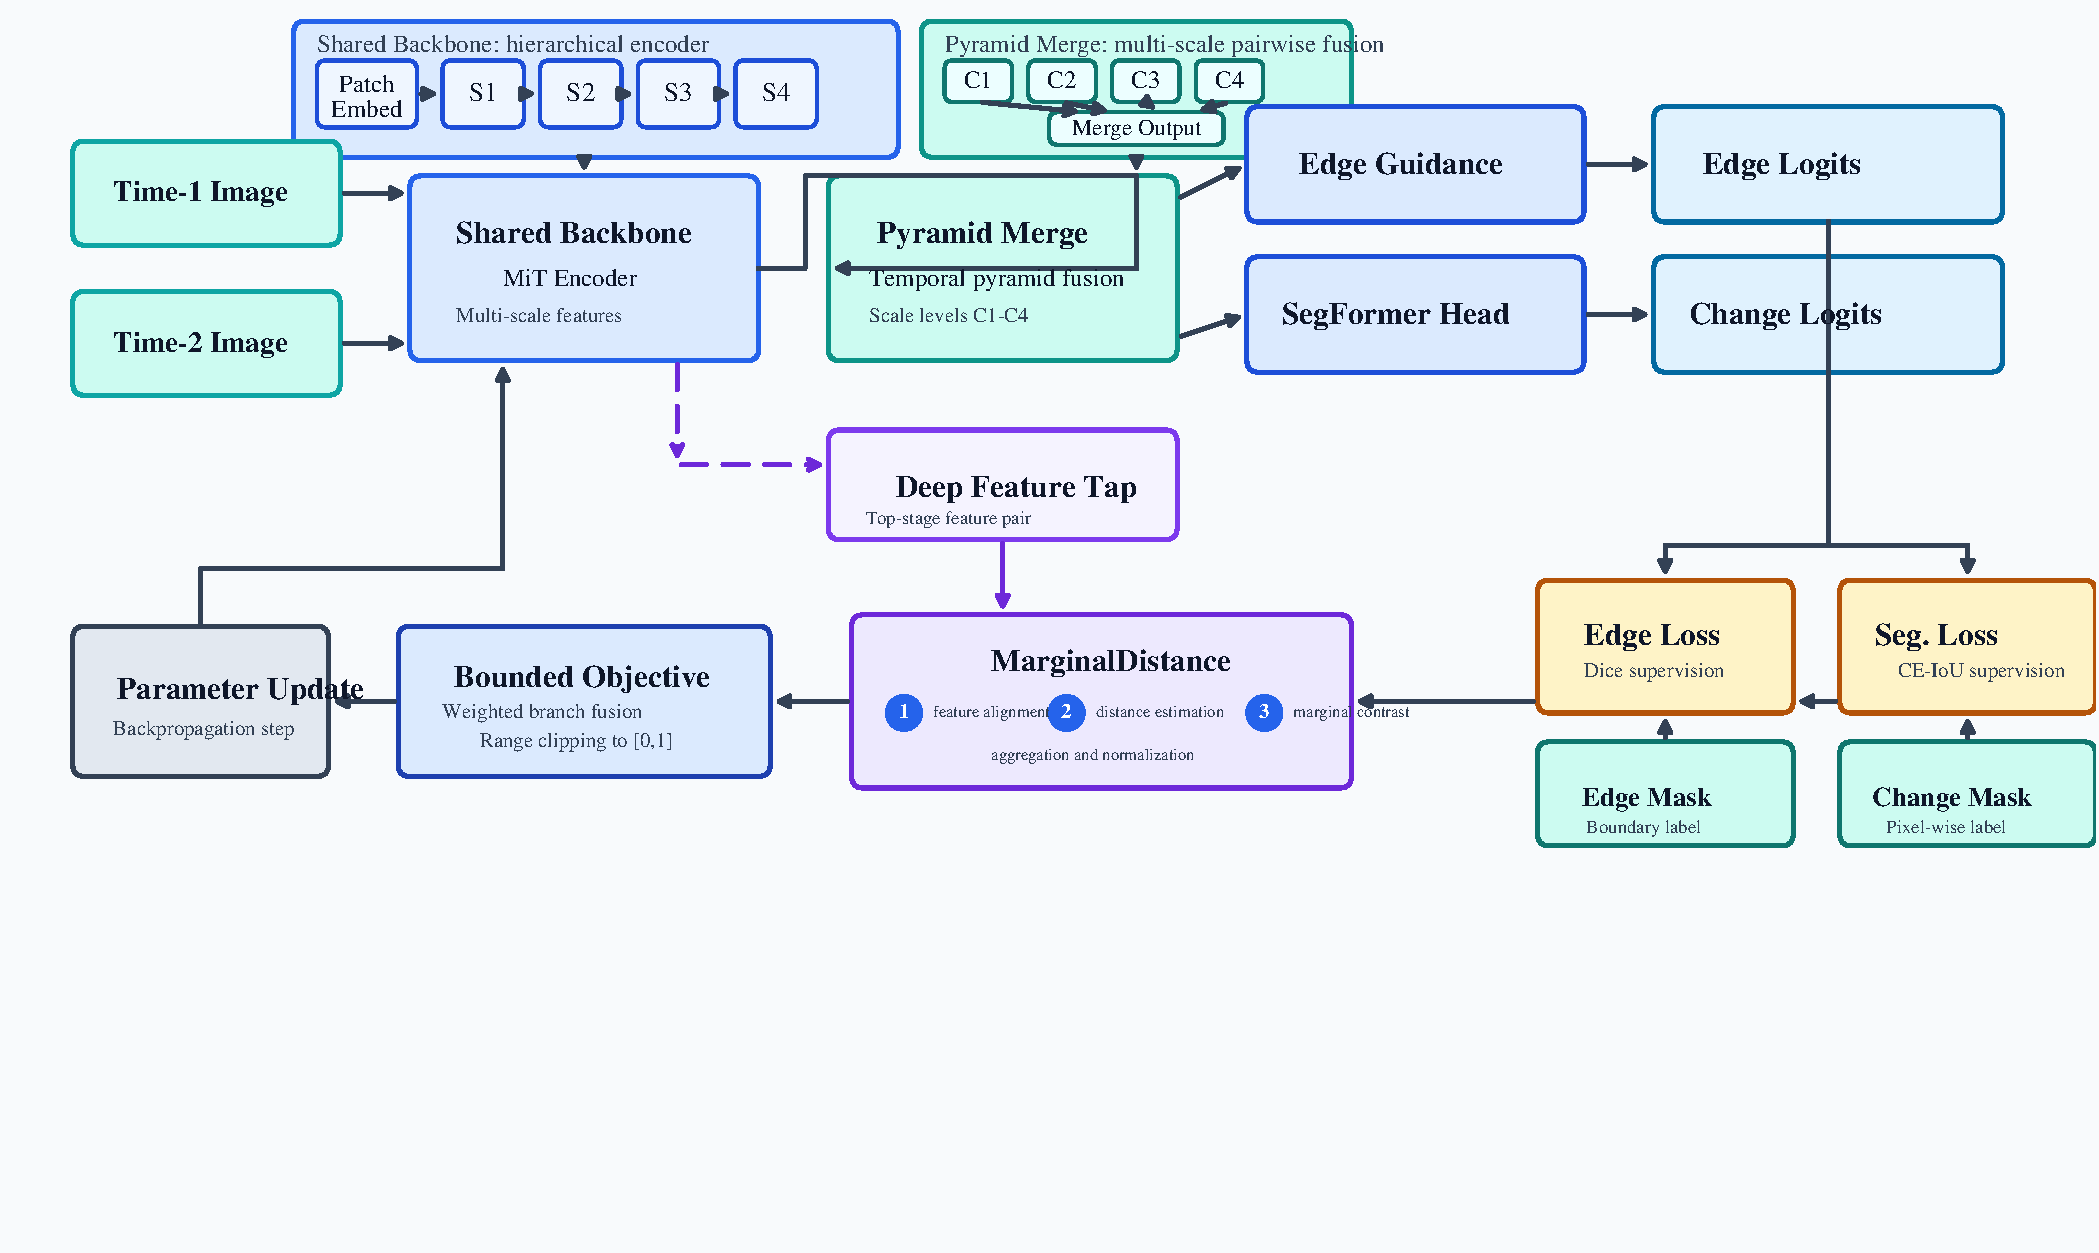
\includegraphics[width=0.98\textwidth]{Figures/overview_method_pipeline.pdf}
    \caption{Overall training pipeline of the proposed method. The model contains shared temporal encoding, pyramid-level fusion, dual prediction heads (change and edge), and a \textsc{MarginalDistance} branch for pseudo-change suppression. Multi-branch losses are bounded and fused to update network parameters.}
    \label{fig:method_overview}
\end{figure*}

Given bi-temporal images $\mathbf{I}^{t_1}$ and $\mathbf{I}^{t_2}$, the network $\mathcal{N}_{\theta}$ outputs change logits $\mathbf{P}$, edge logits $\mathbf{P}^{e}$, and deep features $\mathbf{F}^{t_1},\mathbf{F}^{t_2}$:
\begin{equation}
    \left(\mathbf{P},\mathbf{P}^{e},\mathbf{F}^{t_1},\mathbf{F}^{t_2}\right)
    =
    \mathcal{N}_{\theta}\left(\mathbf{I}^{t_1},\mathbf{I}^{t_2}\right).
    \label{eq:network_mapping}
\end{equation}

Following Fig.~\ref{fig:method_overview}, supervision is organized into three branches: segmentation (CE and IoU), edge prediction, and contrastive discrepancy modeling. Their normalized terms are finally fused into a bounded objective for stable multi-task optimization.

\subsection{Pseudo-Change Suppression via Label-Guided Contrastive Supervision}\label{sec:Methodology:PseudoChangeSuppression}
Let $(i,j)\in\Omega$ denote a pixel location, and let $\mathbf{F}^{t_1},\mathbf{F}^{t_2}\in\mathbb{R}^{C\times H\times W}$ be deep features from the two temporal inputs. We first apply channel-wise L2 normalization:
\begin{equation}
    \tilde{\mathbf{f}}^{t_1}_{ij}=
    \frac{\mathbf{F}^{t_1}_{ij}}{\left\|\mathbf{F}^{t_1}_{ij}\right\|_2},
    \qquad
    \tilde{\mathbf{f}}^{t_2}_{ij}=
    \frac{\mathbf{F}^{t_2}_{ij}}{\left\|\mathbf{F}^{t_2}_{ij}\right\|_2}.
    \label{eq:feature_normalization}
\end{equation}
Then the pixel-wise Euclidean distance is
\begin{equation}
    d_{ij}=\left\|\tilde{\mathbf{f}}^{t_1}_{ij}-\tilde{\mathbf{f}}^{t_2}_{ij}\right\|_2.
    \label{eq:feature_distance}
\end{equation}

With binary label $y_{ij}\in\{0,1\}$ ($0$: unchanged, $1$: changed), the pixel-wise contrastive penalty is
\begin{equation}
    \ell_{\text{con}}^{ij}
    =
    \frac{1-y_{ij}}{2}d_{ij}^{2}
    +
    \frac{y_{ij}}{2}\max(0,m-d_{ij})^{2},
    \label{eq:pixel_contrastive}
\end{equation}
where $m$ is the contrastive margin. Unchanged pixels are pulled closer, while changed pixels are pushed apart up to the margin.

The image-level contrastive loss is
\begin{equation}
    \bar{\mathcal{L}}_{\text{con}}
    =
    \frac{1}{HW}\sum_{i=1}^{H}\sum_{j=1}^{W}\ell_{\text{con}}^{ij},
    \label{eq:image_contrastive}
\end{equation}
and its bounded form is
\begin{equation}
    \mathcal{L}_{\text{con}}^{\text{norm}}
    =
    \operatorname{clip}
    \left(
        \frac{\bar{\mathcal{L}}_{\text{con}}}{\max\left(1,\frac{1}{2}m^2\right)},
        0,1
    \right).
    \label{eq:contrastive_normalization}
\end{equation}

\subsection{Objective Function}\label{sec:Methodology:ObjectiveFunction}
Following Table~\ref{tab:notations}, let $\mathbf{Y}$ be the change label map, $\mathbf{Y}^{e}$ be the edge label map, and $\theta$ be network parameters. The segmentation branch combines CE and IoU losses:
\begin{equation}
    \mathcal{L}_{\text{seg}}
    =
    \alpha\,\mathcal{L}_{\text{ce}}^{\text{norm}}
    +
    (1-\alpha)\,\mathcal{L}_{\text{iou}}^{\text{norm}},
    \label{eq:segmentation_fusion}
\end{equation}
with
\begin{equation}
    \mathcal{L}_{\text{ce}}^{\text{norm}}=1-\exp\left(-\mathcal{L}_{\text{ce}}\right),
    \label{eq:ce_normalization}
\end{equation}
\begin{equation}
    \mathcal{L}_{\text{iou}}^{\text{norm}}=\operatorname{clip}(\mathcal{L}_{\text{iou}},0,1),
    \qquad
    \mathcal{L}_{\text{edge}}^{\text{norm}}=\operatorname{clip}(\mathcal{L}_{\text{edge}},0,1).
    \label{eq:edge_iou_normalization}
\end{equation}

The fused multi-task objective is
\begin{equation}
    \mathcal{L}_{\text{total}}
    =
    (1-\beta-\gamma)\mathcal{L}_{\text{seg}}
    +
    \beta\mathcal{L}_{\text{con}}^{\text{norm}}
    +
    \gamma\mathcal{L}_{\text{edge}}^{\text{norm}},
    \label{eq:total_objective}
\end{equation}
subject to $0\le\beta\le1$, $0\le\gamma\le1$, and $\beta+\gamma\le1$. The final bounded loss is
\begin{equation}
    \mathcal{L}=\operatorname{clip}(\mathcal{L}_{\text{total}},0,1).
    \label{eq:final_objective}
\end{equation}

Accordingly, the optimization target is
\begin{equation}
    \theta^{*}
    =
    \arg\min_{\theta}
    \mathbb{E}_{\left(\mathbf{I}^{t_1},\mathbf{I}^{t_2},\mathbf{Y},\mathbf{Y}^{e}\right)}
    \left[\mathcal{L}\right].
    \label{eq:argmin_objective}
\end{equation}

\subsection{Algorithm: Annotation-Consistent Bounded Multi-Task Optimization}\label{sec:Methodology:Algorithm}
Algorithm~\ref{alg:proposed} gives the complete optimization routine. The algorithm explicitly includes forward mapping, contrastive subroutine, bounded loss fusion, and gradient update. Variable semantics are explained inline at first appearance so the flow remains self-explanatory.

\begin{algorithm}[t]
    \caption{Annotation-Consistent Bounded Multi-Task Optimization}
    \label{alg:proposed}
    \begin{algorithmic}[1]
        \Require bi-temporal images $\mathbf{I}^{t_1},\mathbf{I}^{t_2}$; change labels $\mathbf{Y}$; edge labels $\mathbf{Y}^{e}$; contrastive margin $m$; CE/IoU balance $\alpha$; branch weights $\beta,\gamma$; network parameters $\theta$
        \Ensure updated $\theta$ and final bounded loss $\mathcal{L}$
        \State Perform forward mapping to obtain $\mathbf{P}$, $\mathbf{P}^{e}$, $\mathbf{F}^{t_1}$, and $\mathbf{F}^{t_2}$ by Eq.~\eqref{eq:network_mapping}
        \State Compute $\mathcal{L}_{\text{con}}^{\text{norm}}$ using \textsc{MarginalDistance}$(\mathbf{F}^{t_1},\mathbf{F}^{t_2},\mathbf{Y},m)$
        \State Compute $\mathcal{L}_{\text{ce}}$, $\mathcal{L}_{\text{iou}}$, and $\mathcal{L}_{\text{edge}}$ as defined in Section~\ref{sec:Preliminary}
        \State Bound branch losses: $\mathcal{L}_{\text{ce}}^{\text{norm}}$ by Eq.~\eqref{eq:ce_normalization}; $\mathcal{L}_{\text{iou}}^{\text{norm}}$ and $\mathcal{L}_{\text{edge}}^{\text{norm}}$ by Eq.~\eqref{eq:edge_iou_normalization}
        \State Compute $\mathcal{L}_{\text{seg}}$ by Eq.~\eqref{eq:segmentation_fusion}
        \State Compute $\mathcal{L}_{\text{total}}$ by Eq.~\eqref{eq:total_objective}
        \State Compute final bounded loss $\mathcal{L}$ by Eq.~\eqref{eq:final_objective}
        \State Update $\theta$ via backpropagation with objective $\mathcal{L}$
        \Statex
        \Procedure{MarginalDistance}{$\mathbf{F}^{t_1},\mathbf{F}^{t_2},\mathbf{Y},m$}
            \State Define pixel-coordinate set $\Omega$
            \For{each $(i,j)\in\Omega$}
                \State Normalize $\mathbf{F}^{t_1}_{ij}$ and $\mathbf{F}^{t_2}_{ij}$ to unit vectors by Eq.~\eqref{eq:feature_normalization}
                \State Compute feature distance $d_{ij}$ by Eq.~\eqref{eq:feature_distance}
                \State Compute pixel penalty $\ell_{\text{con}}^{ij}$ by Eq.~\eqref{eq:pixel_contrastive} with label $y_{ij}\in\{0,1\}$
            \EndFor
            \State Average over pixels to obtain $\bar{\mathcal{L}}_{\text{con}}$ by Eq.~\eqref{eq:image_contrastive}
            \State Normalize and clip $\bar{\mathcal{L}}_{\text{con}}$ to $\mathcal{L}_{\text{con}}^{\text{norm}}$ by Eq.~\eqref{eq:contrastive_normalization}
            \State \Return $\mathcal{L}_{\text{con}}^{\text{norm}}$
        \EndProcedure
    \end{algorithmic}
\end{algorithm}

    
    % 实验
    \section{Experiment}\label{sec:Experiment}
    Write the Experiment parts here.%写一个阶段实验章的开场白
    \subsection{Implementation Details}\label{subsec:Implementation Details}%实验细节
        \paragraph{Datasets.} We evaluate on four widely-used change detection datasets: LEVIR-CD, WHU-CD, GZ-CD, and CLCD. These datasets cover various geographic regions, land cover types, and change patterns, providing a comprehensive testbed for cross-dataset generality.%后续自己重写数据集描述：简介，引用，

        \paragraph{Evaluation Metrics.} We report six metrics: Precision (Pre), Recall (Rec), F1-score (F1), Intersection over Union (IoU), Overall Accuracy (OA), and Kappa coefficient. These metrics capture different aspects of detection quality, including pixel-wise classification, region overlap, and agreement beyond chance.%后续自己重写指标描述：简介，公式，意义

        \paragraph{Model Details.} The model details, training settings, and other implementation specifics will be described in the next sections.%网络模型的介绍，对比方法中所用的神经网络模型，

        \paragraph{Hyperparameters.} % 主要超参的值，可以用表格的形式

        \paragraph{Hardware Details.} % 介绍服务器处理器显卡内存信息系统等硬件环境信息
    

    \subsection{Main Results}\label{subsec:Main Results}%表格呈现本方法与主要对比方法的结果同时需要针对表格有一段量化分析讨论的表述


    \subsection{Results on Pseudo-Change Datasets}\label{subsec:Results on Pseudo-Change Datasets}%表格形式在伪变化数据集上与主流方法作对比同时针对表格有一段量化分析讨论的表述


    \subsection{Ablation Study}\label{subsec:Ablation Study}%表格形式展示消融实验结果同时针对表格有一段量化分析讨论的表述


    \subsection{Visualization Analysis}\label{subsec:Visualization Analysis}%可视化结果展示同时针对可视化结果有一段分析讨论的表述,用来挑选对我有利的可视化结果，展示我方法在伪变化抑制和边界优化方面的优势


    \subsection{Model Complexity and Efficiency}\label{subsec:Model Complexity and Efficiency}%表格形式展示模型复杂度和效率结果同时针对表格有一段量化分析讨论的表述，训练的时间、显存的开销，推理的时间和显存的开销等 推理时间、参数量，python包calops等工具计算模型的复杂度和效率指标,统计模型的参数量、FLOPs、训练时间、推理时间等指标，并与对比方法进行比较，分析模型在实际应用中的效率和可行性。


    \subsection{Discussion}\label{subsec:Discussion}%对实验结果的总结和分析，强调我方法在伪变化抑制和边界优化方面的优势，同时也指出可能的不足和未来的改进方向
        


    
    % 结论
    \section{Conclusion}\label{sec:Conclusion}
    The conclusion goes here.       
    
    % 致谢、项目、基金
    \input{Sections/7-Acknowledgments}    
    
    % 附录
    {\appendix

\section*{Proof of the Zonklar Equations}\label{appdx:Proof}
    Use $\backslash${\tt{appendix}} if you have a single appendix:
    Do not use $\backslash${\tt{section}} anymore after $\backslash${\tt{appendix}}, only $\backslash${\tt{section*}}.
    If you have multiple appendixes use $\backslash${\tt{appendices}} then use $\backslash${\tt{section}} to start each appendix.
    You must declare a $\backslash${\tt{section}} before using any $\backslash${\tt{subsection}} or using $\backslash${\tt{label}} ($\backslash${\tt{appendices}} by itself
     starts a section numbered zero.)

\section*{ABc}\label{appdx:ABC}

}    
    
    % 引用文献列表
    \bibliographystyle{IEEEtran}  % 选择 IEEE 的引用样式
    \bibliography{references}    % 这里是你的 .bib 文件的名字，不需要加扩展名    
    
    \newpage    
    
    % 作者简介。    
    \input{Sections/9-Biography}    

\end{document}
